\chapter{Simulation Setup and Validation} \label{ch:sim_setup} 

\section{3D Molecular Dynamics Simulation} \label{sec:md_setup}

\subsection{Construction of the Copper fcc Lattice Structure}

The construction of the MD simulation began by implementing the copper lattice model through a set of equilibrium lattice points. An fcc lattice was defined using the primitive basis vectors

\begin{align}
	\vec{b}_1 = a\left(1,1,0\right), \nonumber \\
	\vec{b}_2 = a\left(1,0,1\right), \label{eq:primitive_basis_vectors} \\
	\vec{b}_3 = a\left(0,1,1\right). \nonumber
\end{align}
\\
The lattice parameter $a=1.80\si{\angstrom}$ was used, consistent with the lattice parameter of copper measured using x-ray crystallography \cite{davey}.
Harmonic nearest neighbour forces were implemented with force constant $k=\SI{28}{\newton\per\metre}$. This configuration has been shown to reproduce the phonon spectrum of copper \cite{sinha}. Periodic boundary conditions were imposed in the $\left[1,0,\bar{1}\right]$-$\left[0,1,\bar{1}\right]$ plane and the bottom layer of the substrate in the $\left[1,1,1\right]$ direction was was held fixed at its equilibrium position to prevent undesirable center of mass motion of the crystal. The top layer in the $\left[1,1,1\right]$ direction (which corresponds to a 111 surface for an fcc crystal) was left as a free surface on which a single adatom could be placed. The physical structure of the substrate is summarized in Figure \ref{fig:crystal_structure}.

\begin{figure}
	\begin{subfigure}[t]{0.45\textwidth}
		\centering
		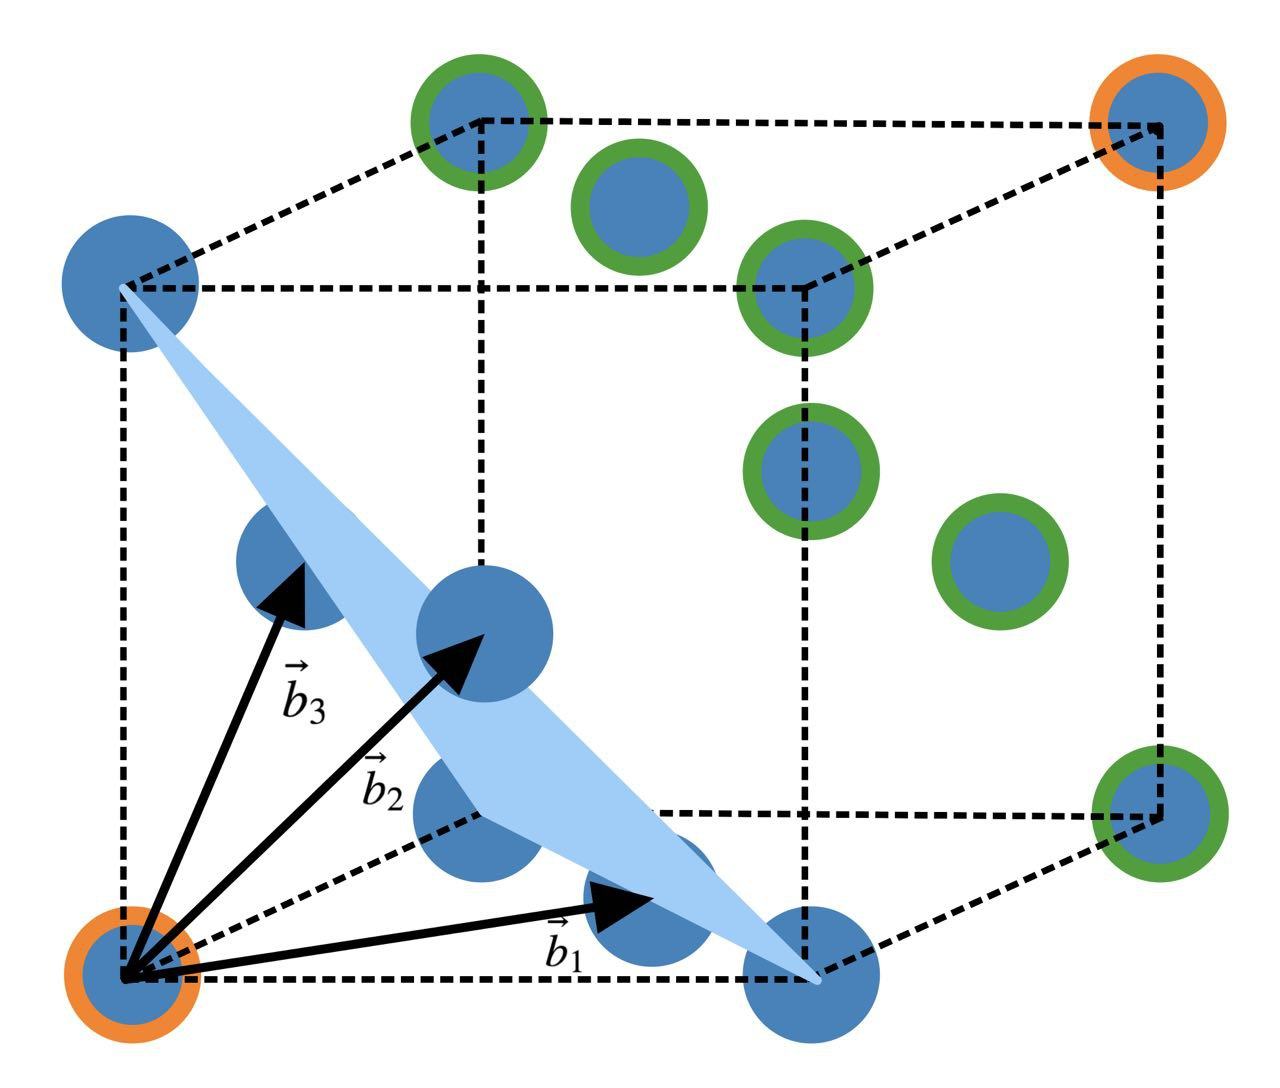
\includegraphics[width=1.0\textwidth]{fcc_cell}
		\caption{The form of the fcc crystal structure used in the simulation. Annotates the definitions of $\vec{b}_i$ in equation \ref{eq:primitive_basis_vectors} as well as the fcc 111 plane.} \label{fig:fcc_cell} 
	\end{subfigure}
	\hfill
	\begin{subfigure}[t]{0.45\textwidth}
		\centering
		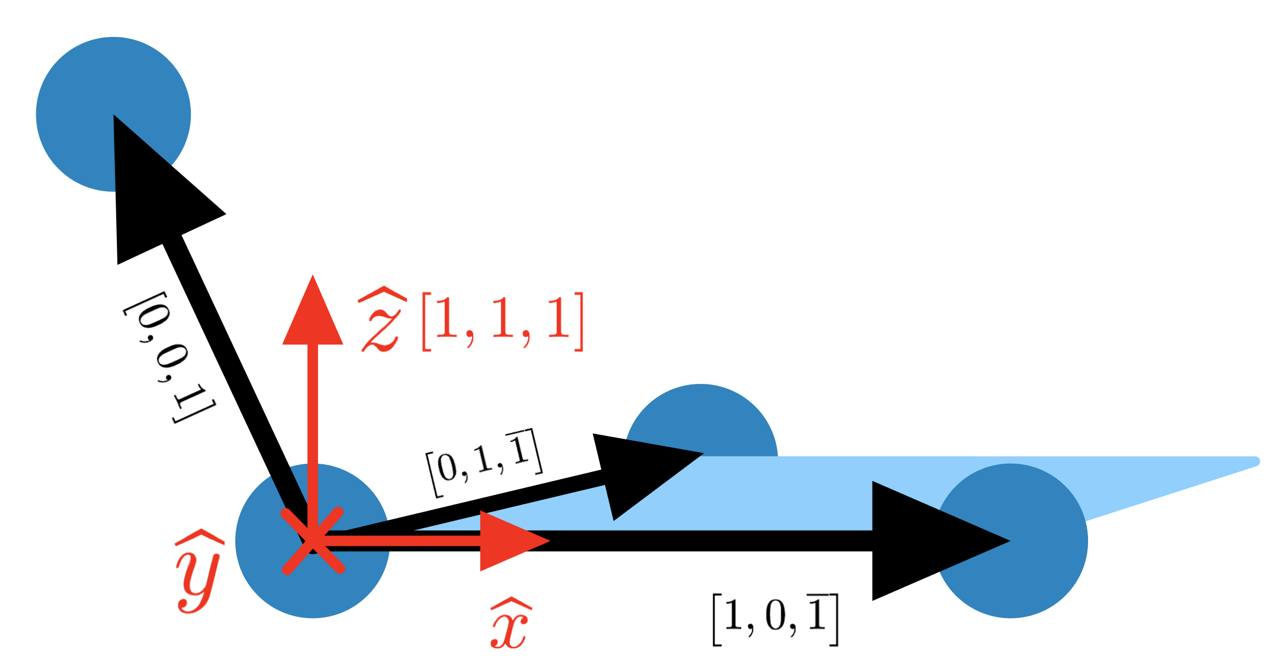
\includegraphics[width=1.0\textwidth]{in_plane_basis}
		\caption{Depicts the $\left[1,0,\bar{1}\right]$, $\left[0,1,\bar{1}\right]$ $\left[0,0,1\right]$ \& $\left[111\right]$ directions after rotating the crystal to align the 111-plane with the xy-plane.\label{fig:in_plane_basis}}
	\end{subfigure}
	\hfill
	\begin{subfigure}[t]{0.45\textwidth}
		\centering
		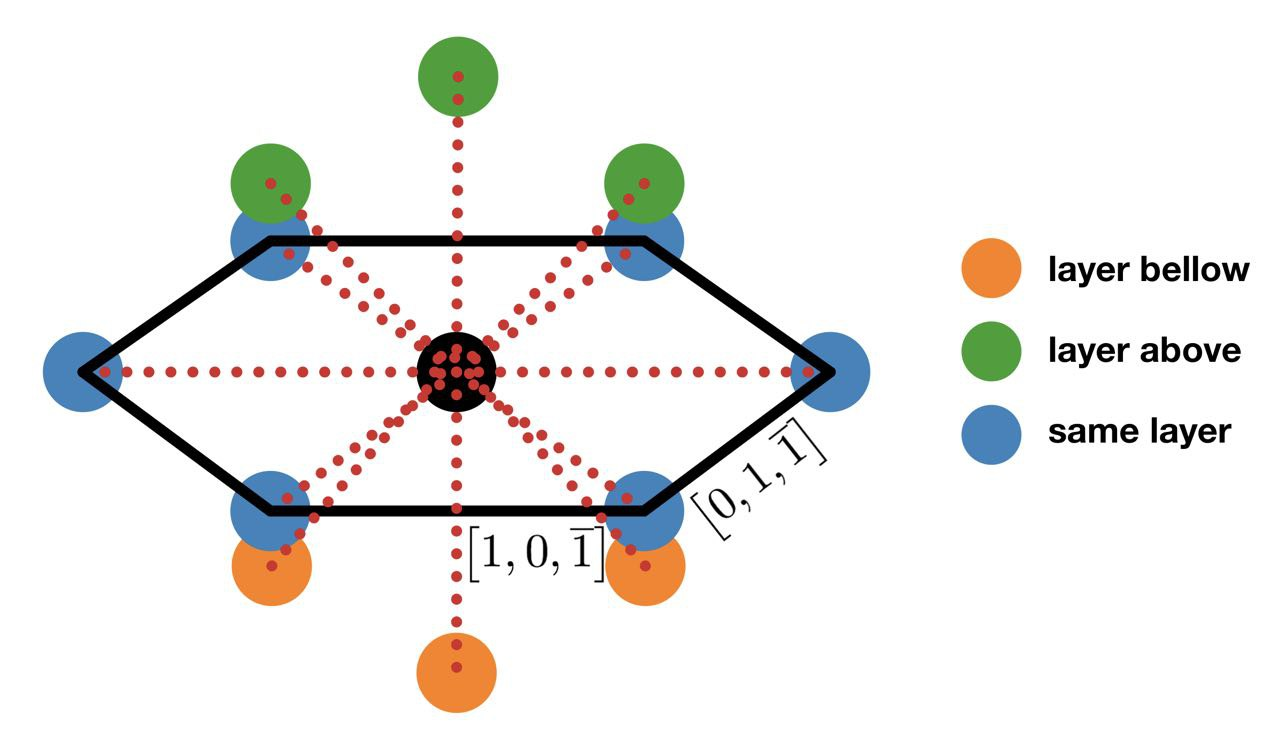
\includegraphics[width=1.0\textwidth]{nearest_neighbours}
		\caption{Each atom in the crystal is connected to its twelve nearest neighbors with a spring of natural length equal to the nearest neighbor distance of the fcc crystal ($2.54\angstrom$).} \label{fig:nearest_neighbours}	
	\end{subfigure}
	\hfill
	\begin{subfigure}[t]{0.45\textwidth}
		\centering
		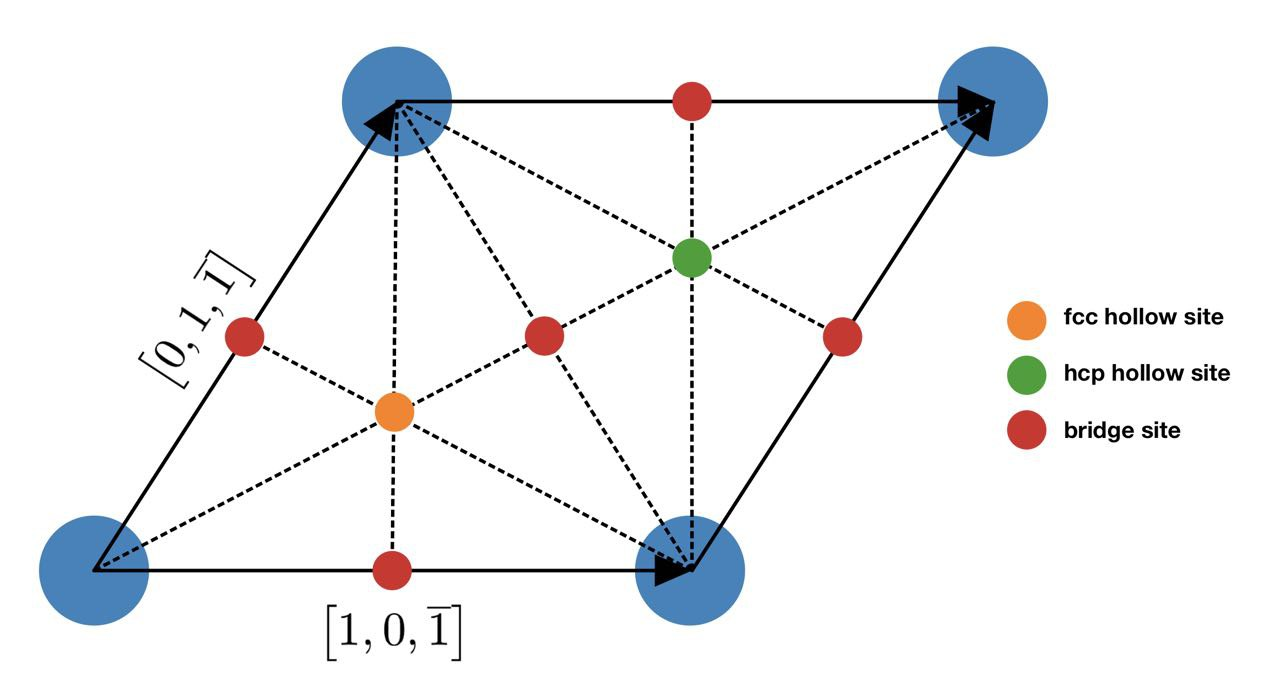
\includegraphics[width=1.0\textwidth]{primitive_cell}
		\caption{The top 111-plane in the crystal is tiled by the shown unit cell.} \label{fig:in_plane_cell}
	\end{subfigure}
\caption{Depiction of the fcc crystal structure with lattice parameter $1.8\angstrom$ used in the simulation to model a copper crystal with a free 111 plane.}
\label{fig:crystal_structure}
\end{figure}

\subsection{Adsorbate Substrate Interactions}

\begin{figure}
	\centering
	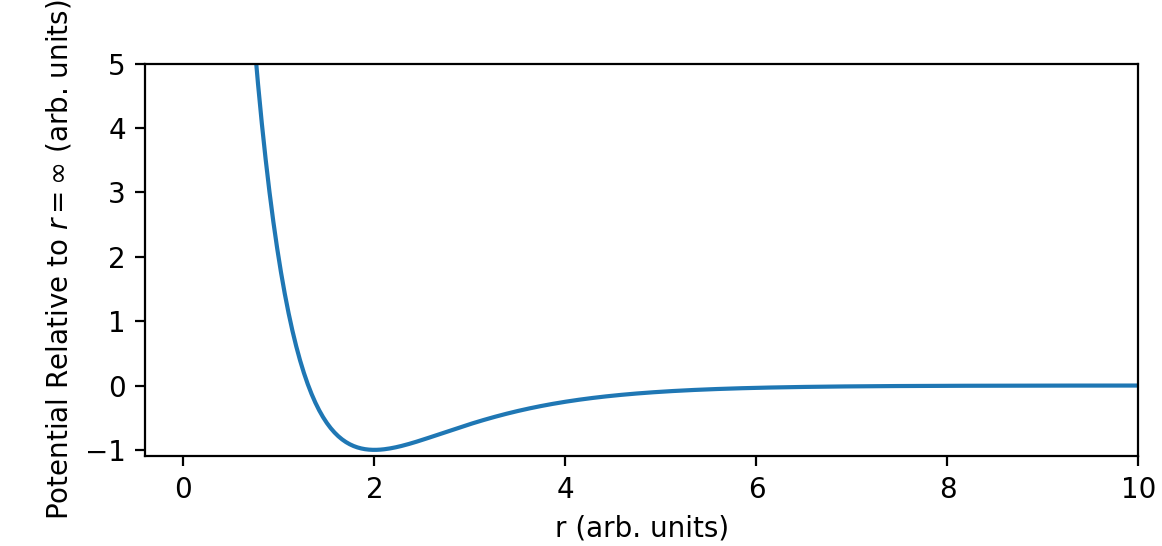
\includegraphics[width=0.8\textwidth]{morse_potential}
	\caption{The typical shape of a Morse potential as a function of particle separation.}
	\label{fig:morse_potential}
\end{figure}

A Morse potential (Figure \ref{fig:morse_potential}) was chosen for the adatom-substrate interaction given by the formula 
\begin{equation}
	V\left(r\right) = D(1-e^{-a\left(r-r_0\right)})^2 \label{eq:morse}
\end{equation}
where $D,a$ and $r_0$ are free parameters which control the depth, width and position of the potential well. This is a common choice for MD simulations \cite{SHUSTOROVICH19981, ELLIS199499}. For computational efficiency, at each simulation time-step, only substrate atoms within $4.5 \times r_0$ of the adatom (modulo the periodic boundary conditions) were included in the interaction. 

\subsection{Initializing and Propagating the Simulation}

In order to achieve the desired equilibrium temperature, the equipartition theorem requires the total amount of energy in the system equal $\frac{1}{2}N_{\text{dof}}kT$. The simulation was therefore initialized with all atoms at their equilibrium positions and the initial value of each velocity component sampled from a Gaussian with zero mean and variance $2 \cdot \frac{kT}{m}$. The center of mass velocity of the system was subtracted off to remove unwanted oscillations of the whole substrate off the fixed bottom layer.

At each time-step, the simulation was updated using a Velocity Verlet integrator. This method is commonly used in simulations in which the forces only depend on the positions of the particles involved \cite{Omelyan, Choi}. This gives a set of update equations
\\
$$
	\vec{x}_{n+1} = \vec{x}_n + \vec{v}_n \Delta{t} + \frac{1}{2m}\vec{F}\left(\vec{x}_n\right) \Delta{t}^2
$$
\begin{equation}
	\vec{v}_{n+1} = \vec{v}_n + \frac{1}{2m} \left(\vec{F}\left(\vec{x}_n\right) + \vec{F}\left(\vec{x}_{n+1}\right)\right) \Delta{t}
\end{equation}
\\
which were solved for each particle using a program written in Python 3.7. The operations were vectorized using the numpy library \cite{harris2020array} to ensure the program executed at reasonable speeds while written in Python. The simulation was found to be stable using a time-step of $\Delta{t}=10\si{\femto\second}$, consistent with the result found in \cite{ELLIS199499}. 

\section{Validation of the 3D Molecular Dynamics Simulation}

\subsection{Oscillations near equilibrium}

The first check on the implementation of the MD simulation was performed by setting up a small piece of substrate with two atoms. One atom was held in place in the bottom layer and the other was allowed to oscillate freely. The oscillations of the free atom remained radial with an angular frequency consistent with a spring constant of $28\si{\newton\per\metre}$.

A similar check was performed with an adatom and a single substrate atom which was held in place. The frequency of oscillation for small displacements was found to be consistent with the curvature of the Morse potential at the equilibrium position.

\subsection{Substrate Phonon Spectrum} \label{sec:phonon_spectrum}

\begin{figure}
	\centering
	\begin{subfigure}[t]{0.32\textwidth}
		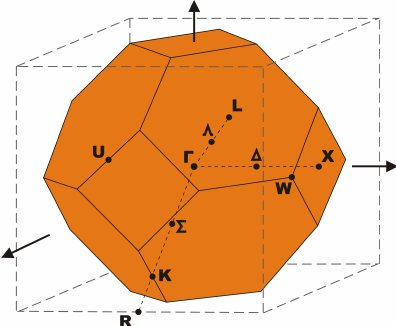
\includegraphics[width=1.0\textwidth]{fcc_brillouin_zone}
		\caption{The fcc Brillouin zone notation used in Figure \ref{fig:experimential_phonon_dispersion_plot} \& \ref{fig:phonon_dispersion_plot} \cite{Zaleski}.}
		\label{fig:fcc_notation}
	\end{subfigure}
	\hfill
	\begin{subfigure}[t]{0.63\textwidth}
		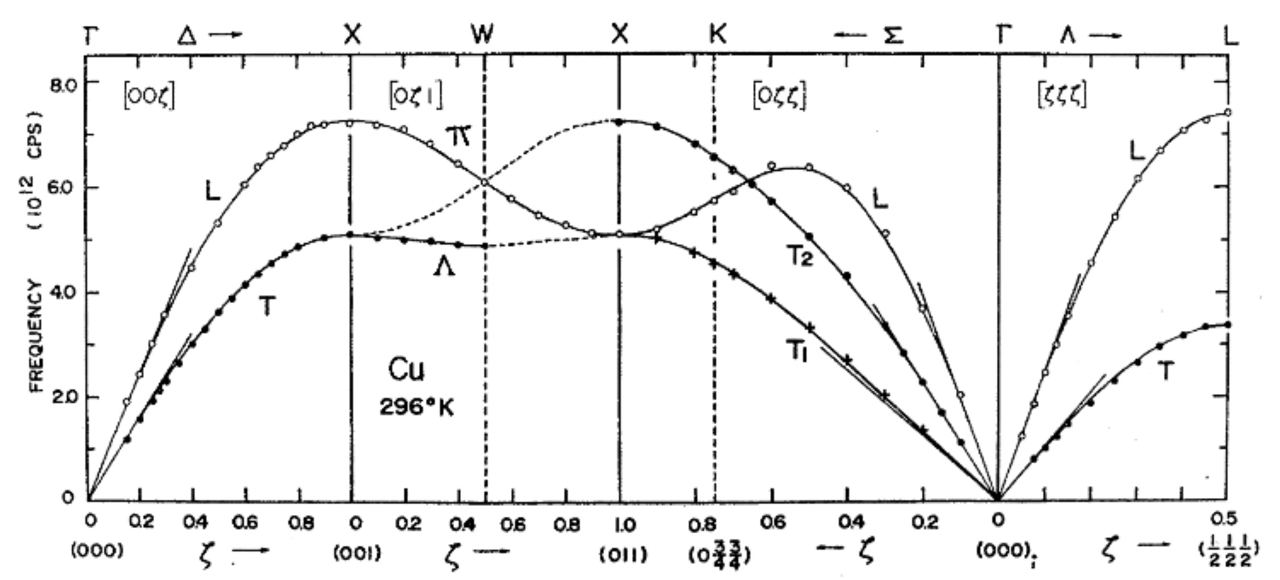
\includegraphics[width=1.0\textwidth]{copper_bulk_phonon_dispersion_curve}
		\caption{The phonon dispersion curves of copper extracted from neutron scattering data at $296\si{\kelvin}$ \cite{Svensson}.}
		\label{fig:experimential_phonon_dispersion_plot}
	\end{subfigure}
	\begin{subfigure}[t]{1.0\textwidth}
		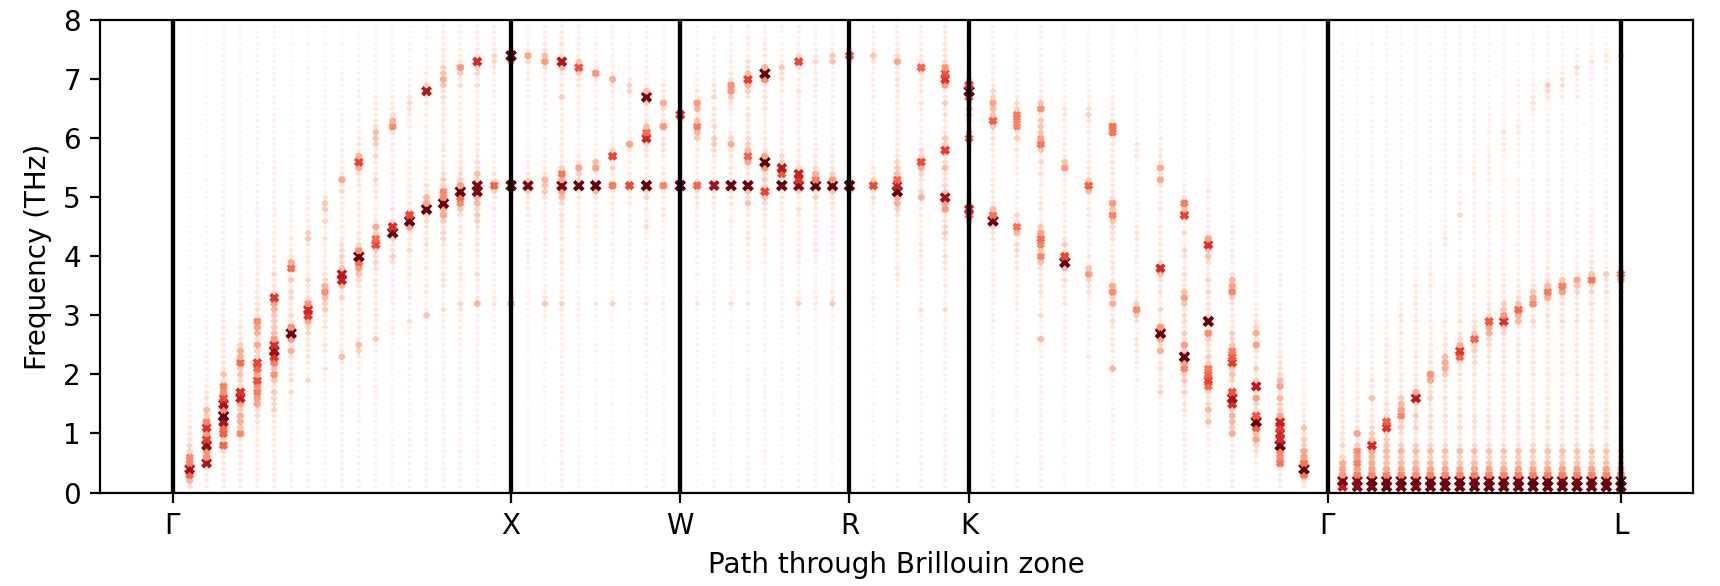
\includegraphics[width=1.0\textwidth]{phonon_dispersion_plot}
		\caption{A substrate phonon dispersion plot extracted from the simulation at $296\si{\kelvin}$ with no adsorbates present. Substrate distortions due to the pinned bottom layer are visible in the $\Gamma\rightarrow \mathrm{L}$ direction.}
		\label{fig:phonon_dispersion_plot}
	\end{subfigure}
	\caption{}
	\label{fig:phonons}
\end{figure}

The implementation of the substrate's structure and periodicity was validated by comparing the phonon spectrum observed in the simulated lattice to the known phonon spectrum in copper shown in Figure \ref{fig:experimential_phonon_dispersion_plot} \cite{sinha}. 

The simulation was run with a $40\times40\times40$ substrate and no adsorbates present for $100\si{\pico\second}$ at $296\si{\kelvin}$. A sequence of k-vectors was defined using a path through the fcc Brillouin zone to match Figure \ref{fig:experimential_phonon_dispersion_plot} as per the fcc Brillouin zone notations in Figure \ref{fig:fcc_notation}. Using this sequence of k-vectors, Figure \ref{fig:phonon_dispersion_plot} was produced using the last $10\si{\pico\second}$ of the run and the formula
\begin{equation}
	A_{\text{phonon}}\left(\vec{k}, f\right) = \int dt \exp\left(-2\pi i ft\right) \sum_{n,k,l=1}^{N,K,L}\sum_{i=1}^3\exp\left(-\vec{k}\cdot\vec{r}_{n,k,l}\right)\left(\vec{\epsilon}_i\cdot\Delta\vec{r}_{n,k,l}\left(t\right)\right)
\end{equation}
\\
where $\vec{k}$ and $f$ are the wave-vector and frequency of a candidate phonon, $\vec{\epsilon}_i$ are three unit vectors spanning the phonon's polarization space, $\vec{r}_{n,k,l}$ is the equilibrium position of the atom with index $n,k,l$ and $\Delta\vec{r}_{n,k,l}$ is its displacement vector. The large red crosses in Figure \ref{fig:phonon_dispersion_plot} correspond to stable modes of oscillation of the crystal and therefore illuminate the substrate's phonon dispersion curves. These curves demonstrate that the simulation reproduces the physical phonon spectrum of copper in Figure \ref{fig:experimential_phonon_dispersion_plot}. Distortions are clearly visible in the $\Gamma\rightarrow\mathrm{L}$ (corresponding to $\left[111\right]$) direction due to the fixed bottom layer and lack of periodicity in this direction. 

\subsection{Thermodynamic Quantities}


\begin{figure}
	\centering
	\begin{subfigure}[t]{0.48\textwidth}
		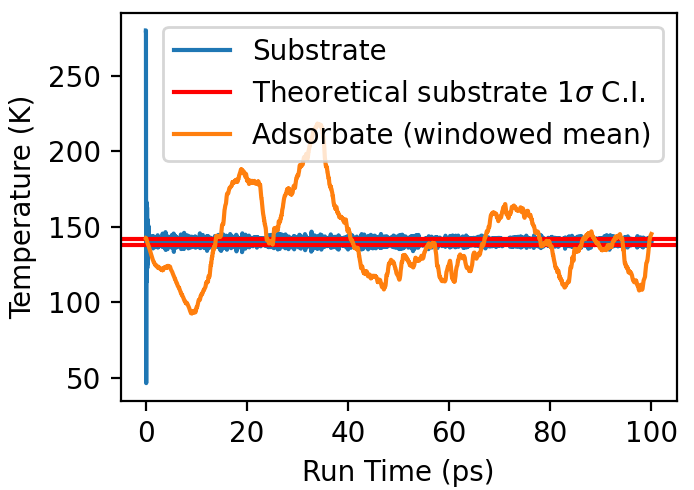
\includegraphics[width=1.0\textwidth]{md_temperature}
		\caption{Temperature as a function of time for the run. The theoretical $\mu \pm 1\bar{\sigma}$ confidence interval accounting for fluctuations of the substrate's kinetic energy is shown in red ($\bar{\sigma}=\sqrt{\frac{5}{3N}}T$).}
		\label{fig:md_temperature}
	\end{subfigure}
	\hfill
	\begin{subfigure}[t]{0.48\textwidth}
		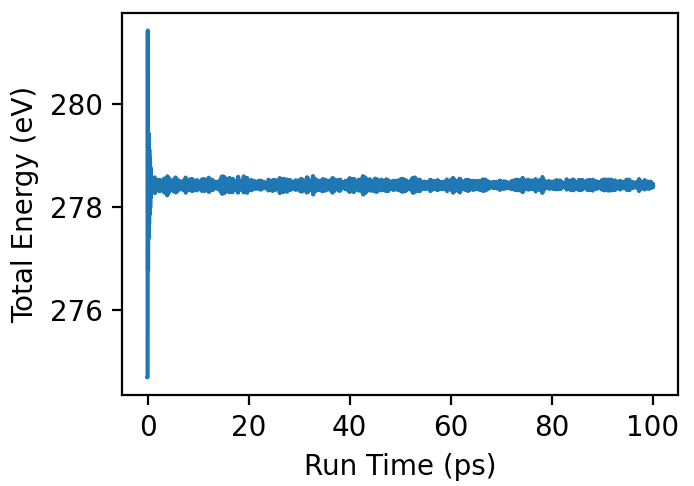
\includegraphics[width=1.0\textwidth]{md_total_energy}
		\caption{Total energy as a function of time. The system is observed to quickly equilibriate with small but bound fluctuations around the equilibrium value due to numerical error.}
		\label{fig:md_total_energy}
	\end{subfigure}
	\begin{subfigure}[t]{0.9\textwidth}
		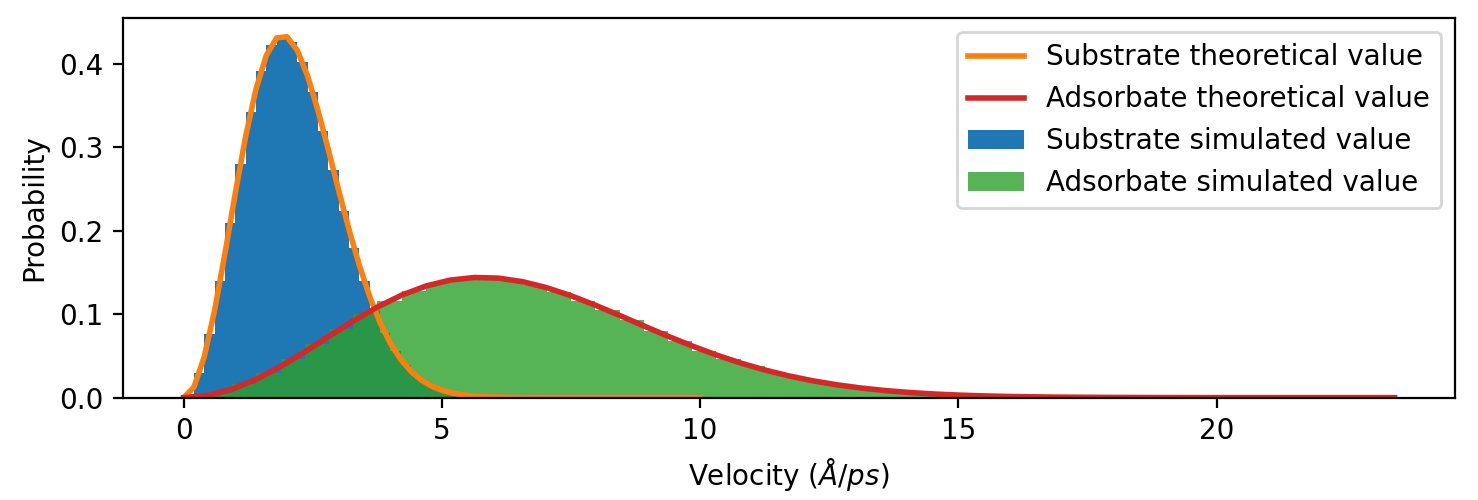
\includegraphics[width=1.0\textwidth]{md_velocities}
		\caption{Histograms of the speed of the adsorbate and substrate particles super-imposed with their respective theoretical 3D Maxwell-Boltzmann distributions.}
		\label{fig:md_velocities}
	\end{subfigure}
	\caption{Example plots of the thermodynamic quantities monitored in each simulation run. The shown run was performed at $140\si{\kelvin}$ for $100\si{\pico\second}$.}
	\label{fig:thermodynamics}
\end{figure}

The temperature, total energy and speed distribution of each simulation run were carefully monitored to ensure that they agreed with their theoretical values. The temperature of the substrate was calculated using the equipartition theorem, $T=\frac{2}{3k}\left<E_k\right>$ where $\left<E_k\right>$ is the average kinetic energy of the substrate atoms. Figure \ref{fig:thermodynamics} shows a typical set of these thermodynamic quantities. All runs reported were found to equilibriate within $1\si{\pico\second}$ and fluctuate around equilibrium within the expected theoretical bounds. All analysis either excluded the first few picoseconds of a run or the simulation was run long enough for the equilibriation period to be considered negligible.

\section{Fitting Simulation Parameters to Experimental Data} \label{sec:md_fit}

\begin{table}[h!]
	\centering
\begin{tabular}{ |p{3.5cm}|p{2.1cm}|p{1.8cm}||p{2.8cm}|p{2.8cm}|}
 \hline
 \multicolumn{5}{|c|}{Results of Parameter Optimization} \\
 \hline
	Feature & Target Value & Fit Value & Morse Parameter & Optimized Value \\
 \hline
	$\left[111\right]$ Vibration Freq. & $38\si{\milli\eV}$ \cite{livibfreq} & $36.2\si{\milli\eV}$ & $D$ & $103.7\mev$ \\
	Equilibrium Height & $2.1\si{\angstrom}$ \cite{PADILLACAMPOS1997183} & $2.2\si{\angstrom}$ & $a$ & $1.527\si{\angstrom}^{-1}$ \\
	FCC/HCP Pot. Diff. & $0\mev$ \cite{Guido,Ward} & $0.4\mev$ & $r_0$ & $2.896\si{\angstrom}$ \\
	Bridge Site Barrier & $9\mev$ \cite{PADILLACAMPOS1997183, Ward} & $9.4\mev$ & & \\
 \hline
\end{tabular}
	\caption{The features of lithium on copper used to fit the Morse parameters in Equation \ref{eq:morse}. The fitting routine was setup to produce properties close in value to those estimated by independent sources. The best fit parameters and their resulting simulated features are also shown.} 
\label{table:fit_parameters}
\end{table}

Having constructed and validated the 3D molecular dynamics simulation, a fitting routine was constructed to optimize the Morse parameters in the simulation to fit various properties of lithium on copper. Given a set of Morse parameters, a routine was setup to determine the equilibrium height and vibration frequency of an adatom in the $\left[111\right]$ direction as well as the potential difference between the two hollow sites in the fcc crystal and the barrier height between them. These properties have been independently estimated for lithium on copper and are summarized in Table \ref{table:fit_parameters}. 

The $\left[111\right]$ vibration frequency was determined by confining the motion of the adatom above a hollow site to the $\left[111\right]$ direction and allowing the adsorbate to oscillate in place. The vibration frequency was then extracted from the peak in the Fourier spectrum of the atom's $\left[111\right]$ coordinate.

The equilibrium height and potential for each hollow/bridge site was determined by similarly pinning the adatom's position over a site and running the simulation for a short time while damping the motion of the system. Once the system had relaxed, the equilibrium height relative to the substrate was read off and the potential energy of the configuration was calculated as the sum of the energy stored in the Morse interactions as well as the energy in the substrate's inter-atomic bonds due to lattice deformations.

Using the target values in Table \ref{table:fit_parameters} a simple weighted squared difference cost function was implemented and a scipy.optimize.minimize \cite{2020SciPy-NMeth} optimizer instance was used to find a set of Morse parameters to minimize the cost function. The outcome of this fitting process is included in Table \ref{table:fit_parameters}. It was found that the Morse $D$ parameter was largely untouched by the optimizer regardless of its initial value. Therefore future work may be able to fit additional properties using this degree of freedom.

\subsection{Extraction of the Potential Energy Surface} \label{sec:extract_potential}


\begin{figure}
	\centering
	\begin{subfigure}[t]{0.48\textwidth}
		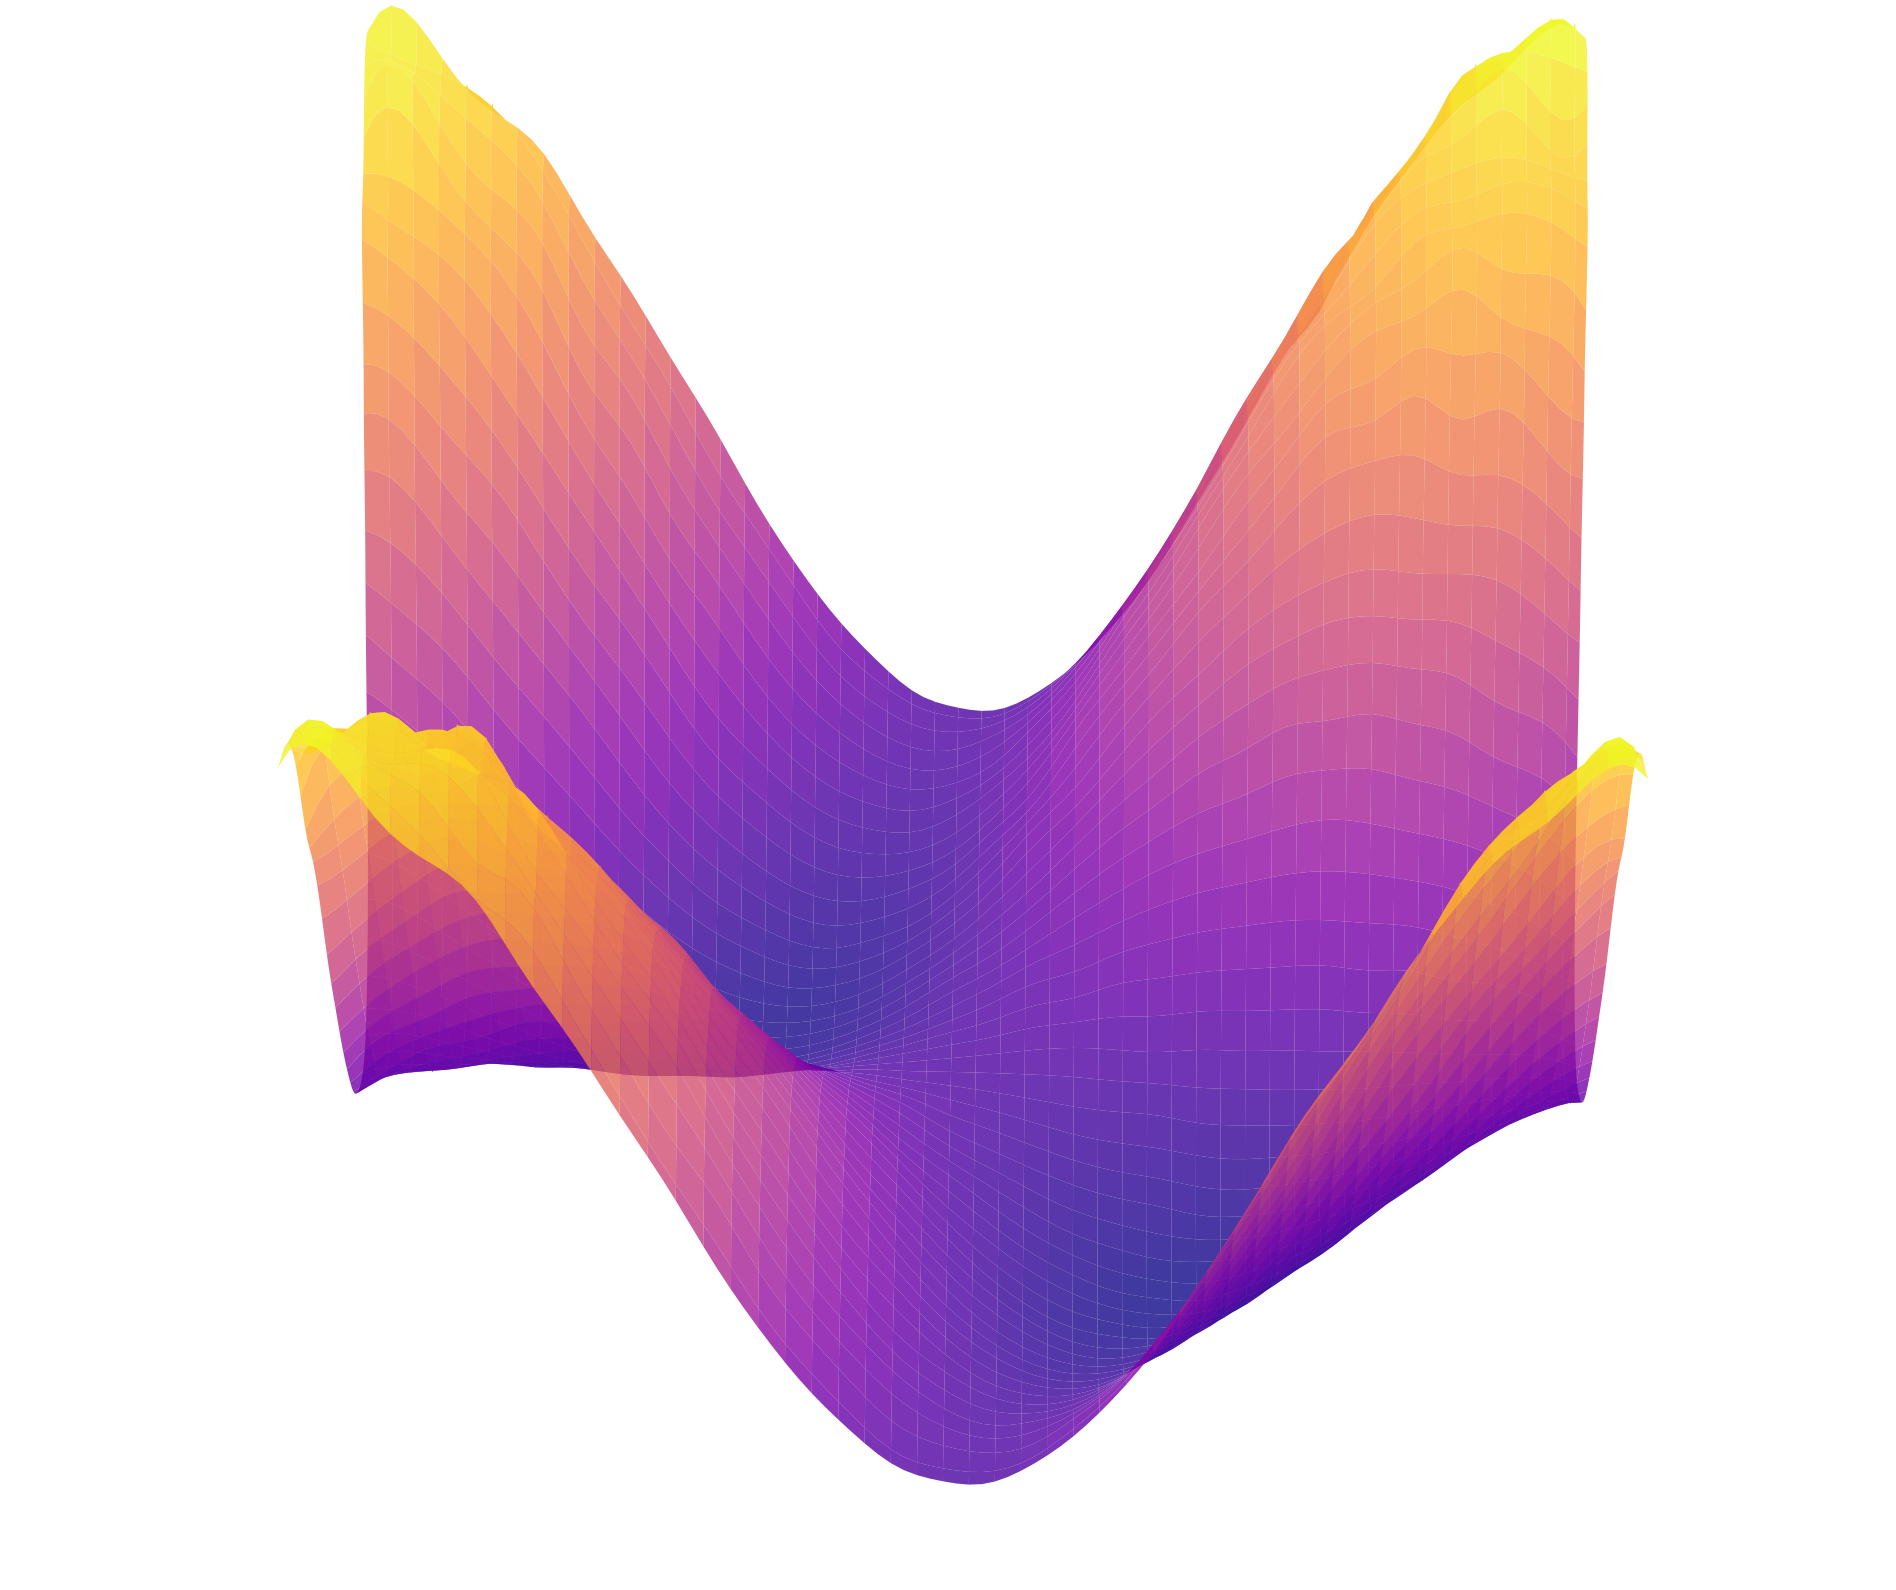
\includegraphics[width=1.0\textwidth]{potential_surface}
		\caption{The 2D potential surface seen by an adatom in the 3D molecular dynamics simulation. Obtained by inverting the Boltzmann factor $P(\vec{x}) \propto e^{-V(\vec{x})/kT}$.}
		\label{fig:potential_surface_plot}
	\end{subfigure}
	\hfill
	\begin{subfigure}[t]{0.48\textwidth}
		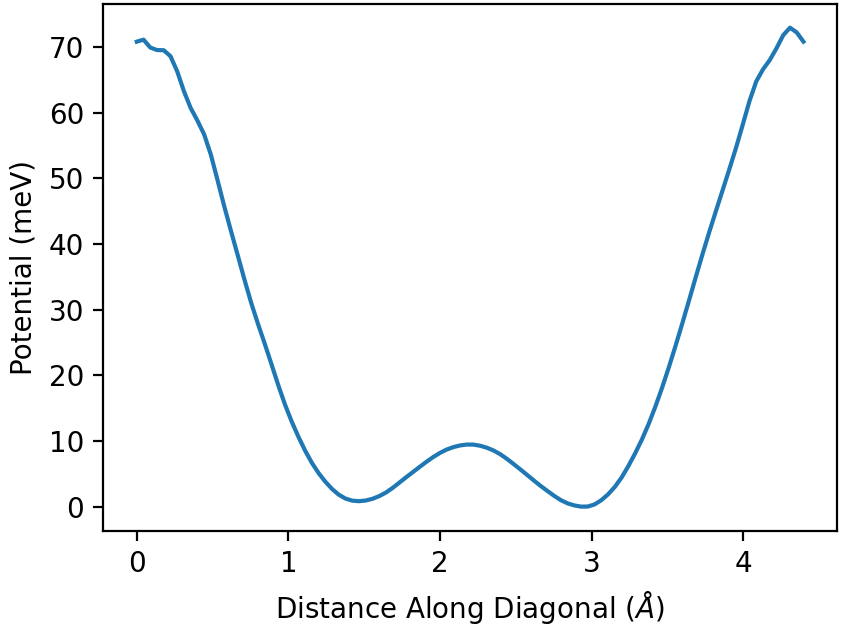
\includegraphics[width=1.0\textwidth]{potential_cross_section}
		\caption{A cross section of the potential surface through the diagonal of Figure \ref{fig:potential_surface_plot}. This exhibits a $9\mev$ barrier height and a $0.4\mev$ fcc/hcp hollow site potential difference.}
		\label{fig:potential_cross_section}
	\end{subfigure}
	\caption{}
	\label{fig:potential_surface}
\end{figure}

The equivalent 2D potential energy surface seen by the adatom in the 3D molecular dynamics simulation was extracted by running the simulation for $100\si{\nano\second}$ with the a $20\times20\times20$ substrate using the parameters in Table \ref{table:fit_parameters}. Each point in the simulated trajectory was mapped back to its equivalent position within the first 2D unit cell on the surface (see Figure \ref{fig:in_plane_cell}). These points were binned on a $30\times30$ grid to provided an estimate of the probability of finding the adatom in each bin at any given time\footnote{Any bins which saw no occupation were assigned an occupation probability of one hundredth of the lowest non-zero occupation probability.}. This probability is proportional to a Boltzmann factor, $P\left(\vec{x}\right) \propto e^{-V\left(\vec{x}\right)/kT}$. This relationship was inverted and the resulting potential surface is shown in Figure \ref{fig:potential_surface}. The statistical noise present on the corners (corresponding to lattice points) was safely ignored since the adatom will very rarely find itself close to these points.

\section{Implementation of the Generalized Langevin Equation Simulations}

A Generalized Langevin Simulation as described in Section \ref{sec:gle_with_background} was constructed using the potential surface extracted from the 3D molecular dynamics simulation shown in Figure \ref{fig:potential_surface}. The $30\times30$ potential grid was interpolated using a scipy.interpolate.RectBivariateSpline \cite{2020SciPy-NMeth} instance and the force at a given position was calculated from the gradient of the potential. 

An exponential memory kernel of the form $K\left(t\right) = \theta(t)\frac{1}{\tau}\exp\left(-\frac{t}{\tau}\right)$ was chosen for its ease of implementation and low computational cost. The discrete memory kernel convolution was implemented using the relation
\\
$$
\int_0^{t_n} dt' K\left(t-t'\right) \vec{f}(t') \approx \alpha \int_0^{t_{n-1}} dt' K\left(t-t'\right) \vec{f}(t') + \frac{1}{1-\alpha} \vec{f}\left(t_n\right)
$$
\\
where $\alpha = \exp{\frac{-\Delta{t}}{\tau}}$ and $\Delta{t}$ is the simulation time-step ($1\si{\femto\second}$ in this case). The normalization factor $\frac{1}{1-\alpha}$ ensures that the total impulse imparted by $\vec{f}(t_n)$ is unaffected by the discretization process. 

The GLE simulations were propagated through time using a Velocity Verlet integrator. Velocity Verlet integration is frequently used in Langevin type simulations \cite{Ward, Townsend}. However, the velocity dependent friction force and non-analytic stochastic force present in Langevin type equations brings into question this choice of integrator \cite{gronbech2013simple}. The performance of the Velocity Verlet integrator and a `modified' Velocity Verlet integrator \cite{Omelyan} in the presence of a background potential are evaluated in Section \ref{sec:thermalization}.

Mention $\tau$ -> $f_c$ correspondance.
